% Propósito: vincular una escala logarítmica de nivel con las presiones
% eficaces correspondientes y mostrar que multiplicar la presión por diez
% agrega 20 dB.
% Origen: L_p=20 log10(p_rms/p_ref), con p_ref=20 microPa,
% ecuación \eqref{eq:u4-nivel-presion}. Los valores son resultados exactos de
% la relación matemática, no umbrales perceptuales ni datos medidos.
% Descripción accesible: una escala horizontal presenta niveles desde 0 hasta
% 120 dB SPL en pasos de 20 dB. Debajo de cada nivel aparece la presión eficaz
% correspondiente, desde 20 micropascales hasta 20 pascales. Cada paso
% multiplica la presión por diez.
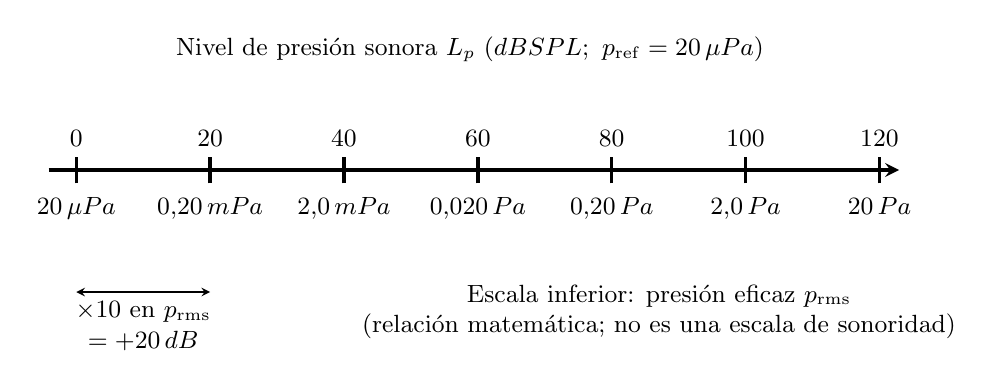
\begin{tikzpicture}[font=\small,>=stealth,x=1cm,y=1cm]
    \draw[->,very thick] (0.75,2.15) -- (11.55,2.15);
    \node[above,align=center] at (6.10,3.40)
        {Nivel de presión sonora \(L_p\)
        \((\text{dB SPL};\ p_\mathrm{ref}=20\,\mu\text{Pa})\)};

    \foreach \x/\lev/\press in {
        1.10/0/{20\,\mu\text{Pa}},
        2.80/20/{0{,}20\,\text{mPa}},
        4.50/40/{2{,}0\,\text{mPa}},
        6.20/60/{0{,}020\,\text{Pa}},
        7.90/80/{0{,}20\,\text{Pa}},
        9.60/100/{2{,}0\,\text{Pa}},
        11.30/120/{20\,\text{Pa}}}{
        \draw[very thick] (\x,1.98) -- (\x,2.32);
        \node[above] at (\x,2.32) {\(\lev\)};
        \node[below,align=center] at (\x,1.93) {\(\press\)};
    }

    \draw[<->] (1.10,0.60) -- (2.80,0.60)
        node[midway,below,align=center]
        {\(\times10\) en \(p_\mathrm{rms}\)\\\(=+20\,\text{dB}\)};
    \node[align=center] at (8.50,0.35)
        {Escala inferior: presión eficaz \(p_\mathrm{rms}\)\\
        (relación matemática; no es una escala de sonoridad)};
\end{tikzpicture}
